\documentclass[11pt,a4paper,reqno]{amsart}
\usepackage[T1]{fontenc}
\usepackage{lmodern}
\usepackage{amsmath,amssymb,mathtools,microtype}
\usepackage[a4paper,margin=30mm]{geometry}
\usepackage{booktabs,enumitem,tikz,xurl}
\usepackage[hidelinks]{hyperref}
\urlstyle{same}
\setlist{nosep}
\setlength{\emergencystretch}{1.5em}
\newtheorem{theorem}{Theorem}[section]
\newtheorem{lemma}[theorem]{Lemma}
\newtheorem{proposition}[theorem]{Proposition}
\newtheorem{corollary}[theorem]{Corollary}
\newtheorem{conjecture}{Conjecture}[section]
\theoremstyle{remark}
\newtheorem{remark}[theorem]{Remark}
\newcommand{\tr}{\operatorname{tr}}
\newcommand{\Spec}{\operatorname{Spec}}
\newcommand{\Ent}{S}
\newcommand{\Pine}{P}
\numberwithin{equation}{section}
\pagestyle{plain}
\title[Minimum von Neumann entropy]{The minimum von Neumann entropy of a connected graph}
% Insert the confirmed authors, affiliations, email addresses, and funding.
% No author or institutional information has been inferred.
\date{}
\subjclass[2020]{05C50, 15A42, 94A17}
\keywords{von Neumann entropy, network structure, graph Laplacian,
R\'enyi entropy, extremal graphs, threshold graphs}
\hypersetup{pdftitle={The minimum von Neumann entropy of a connected graph},
pdfsubject={Mathematics research manuscript},
pdfkeywords={von Neumann entropy, graph Laplacian, threshold graphs}}
\begin{document}
\begin{abstract}
We prove that the star uniquely minimizes the von Neumann entropy
of the trace-normalized combinatorial Laplacian among connected
simple graphs of a given order, confirming Conjecture 1.2 of
Dairyko et al. (2017). Kelmans transformations and an entropy integral
reduce the problem to threshold graphs, where we optimize over the
parameters describing their nested neighbourhoods.
The same method gives sharp bounds with the order, Laplacian rank,
and clique or chromatic number prescribed. The extremal graphs are
pineapple graphs, obtained by attaching leaves to one vertex of a
clique, together with isolated vertices.
A classical comparison between Shannon and R\'enyi entropies also gives
star minimality for every order greater than one, completing
Conjecture 3.3 of Dairyko et al. Among connected nontrees, the triangle pineapple
uniquely minimizes R\'enyi entropy for every finite order at least one. We also derive
the tree extrema from earlier Laplacian coefficient inequalities and
give counterexamples to extensions beyond the stated ranges.
\end{abstract}
\maketitle

\section{Introduction}\label{sec:introduction}

Let $G$ be a finite simple graph with $n$ vertices and $m>0$ edges.
Write $A_G$ for its adjacency matrix, $D_G$ for its diagonal degree
matrix, and $L_G=D_G-A_G$ for its Laplacian matrix. Since $L_G$ is
positive semidefinite and $\tr L_G=2m$, the matrix $\rho_G=L_G/(2m)$
is a density matrix. The interpretation of graph Laplacians as density
matrices was studied by Braunstein, Ghosh, and Severini
\cite{Braunstein2006}; Passerini and Severini \cite{Passerini2009}
subsequently investigated the associated entropy as a measure of
network complexity. If $\mu_1,\ldots,\mu_n$ are the eigenvalues of
$L_G$, the von Neumann entropy of $G$ is
\begin{equation}\label{eq:entropy}
 \Ent(G)=-\tr(\rho_G\log\rho_G)
 =\log(2m)-\frac1{2m}\sum_{i=1}^n\mu_i\log\mu_i,
\end{equation}
where $0\log0=0$. All logarithms in this paper are natural. Division
by $\log2$ gives entropy in bits, the convention used in
\cite{Dairyko2017}.

A different definition of graph entropy uses the symmetric normalized
Laplacian. Minello, Rossi, and Torsello \cite{Minello2019} compared
these two definitions and their quadratic approximations.
Throughout this paper, we use the trace-normalized combinatorial
Laplacian $\rho_G=L_G/(2m)$.

Among nonempty graphs of order $n$, the complete graph maximizes
the entropy, while a single edge together with isolated vertices
minimizes it \cite{Braunstein2006,Dairyko2017}.
Passerini and Severini \cite{Passerini2009} asked whether the star
minimizes entropy among connected graphs of a given order.
Dairyko et al. \cite{Dairyko2017} formulated this as follows.

\begin{conjecture}[Dairyko et al.\ {\cite[Conjecture 1.2]{Dairyko2017}}]\label{conj:star-vonneumann}
If $G$ is connected and has $n\ge2$ vertices, then
$\Ent(G)\ge\Ent(K_{1,n-1})$.
\end{conjecture}

The positive Laplacian eigenvalues of the star are $n$ and $n-2$
copies of $1$. Consequently
$\Ent(K_{1,n-1})=\log(2n-2)-n\log n/(2n-2)$.
Dairyko et al. established sufficient conditions in terms of the
degree sequence and proved that the conjectured inequality holds for
almost all labelled graphs as $n\to\infty$. In particular, they
proved the bound under the density condition
$m/\binom n2\ge1/(\sqrt n-1)$ \cite[Theorem~2.3]{Dairyko2017}.
They also showed that adding an edge can decrease entropy
\cite[Proposition~4.1]{Dairyko2017}, which
prevents a direct reduction to a spanning tree by monotonicity under
edge addition. Lin and Zhou \cite{LinZhou2018} obtained sharp upper
and lower bounds using graph parameters, including the degree and
conjugate degree sequences. These bounds leave open the extremal
problem over all connected graphs. Our main result gives the exact
minimum and its equality case.

\begin{theorem}\label{thm:main}
For every connected simple graph $G$ of order $n\ge2$,
\begin{equation}\label{eq:main}
 \Ent(G)\ge\log(2n-2)-\frac{n\log n}{2n-2}.
\end{equation}
Equality holds if and only if $G\cong K_{1,n-1}$.
\end{theorem}

The main step is an extremal result for threshold graphs.
For $1\le r\le n-1$, let $\Pine(n,r)$ be the graph obtained
from $K_{r+1}$ by attaching $n-r-1$ leaves to one clique vertex.
We call this a pineapple graph. Its nonzero Laplacian spectrum is
$n,(r+1)^{(r-1)},1^{(n-r-1)}$, with multiplicities in parentheses.
In particular, $\Pine(n,1)=K_{1,n-1}$.

\begin{theorem}\label{thm:threshold}
Among connected threshold graphs of order $n$ and clique number $r+1$,
$\Pine(n,r)$ uniquely minimizes von Neumann entropy. For fixed $n$,
the values $\Ent(\Pine(n,r))$ strictly increase with $r$.
\end{theorem}

Theorem~\ref{thm:threshold} also yields sharp bounds with prescribed
graph parameters. If $G$ has $k$ connected components,
put $s=n-k+1=\operatorname{rank}L_G+1$. For either
$r=\omega(G)-1$ or $r=\chi(G)-1$, we prove
\begin{equation}\label{eq:intro-parameter-bound}
 \Ent(G)\ge\log\bigl(2s-2+r(r-1)\bigr)
 -\frac{s\log s+(r^2-1)\log(r+1)}{2s-2+r(r-1)}.
\end{equation}
In each case equality holds precisely for
$\Pine(s,r)\sqcup(k-1)K_1$. The chromatic-number bound requires a
restricted graph transformation: a general Kelmans transformation
can decrease the chromatic number.

The main theorem also implies the R\'enyi entropy conjecture in \cite{Dairyko2017}.
For $\alpha>0$, $\alpha\ne1$, define
$H_\alpha(G)=(1-\alpha)^{-1}\log\tr(\rho_G^\alpha)$ and set
$H_1(G)=\Ent(G)$.

\begin{conjecture}[Dairyko et al.\ {\cite[Conjecture 3.3]{Dairyko2017}}]\label{conj:star-renyi}
For each $\alpha>1$, every connected graph $G$ of order $n\ge2$
satisfies $H_\alpha(G)\ge H_\alpha(K_{1,n-1})$.
\end{conjecture}

The case $\alpha=2$ was proved in \cite[Theorem 3.8]{Dairyko2017}.
Together with the comparison in \cite[Theorem 3]{Harremoes2009},
that result also implies star minimality, with uniqueness, for every
finite $\alpha>2$. Thus the additional range required to complete
Conjecture~\ref{conj:star-renyi} is $1<\alpha<2$.
We give a uniform proof for all $\alpha>1$, including uniqueness, using
Theorem~\ref{thm:main} and a classical extremal comparison between
Shannon and R\'enyi entropies
\cite{Harremoes2009,SakaiIwata2016}. We give a direct proof of the
comparison in the form required here. The conclusion also holds at
$\alpha=\infty$, where $H_\infty(G)=-\log\lambda_{\max}(\rho_G)$.
Among connected nontrees, the triangle pineapple
$U_n=\Pine(n,2)$ uniquely minimizes $H_\alpha$ for every finite
$\alpha\ge1$. We describe the additional equality case at infinite
order separately.

Dairyko et al.\ also conjectured that the path $P_n$ maximizes
von Neumann entropy among trees of order $n$
\cite[Conjecture 1.3]{Dairyko2017}. This inequality already follows
from the Laplacian power-sum bounds of Akbari et al.\
\cite[Corollary 7]{Akbari2010}: all trees of
order $n$ have trace $2n-2$, so normalization and the limit
$\alpha\uparrow1$ give the asserted entropy inequality. The
underlying coefficient ordering was established by Zhou and Gutman
\cite[Theorems 7 and 8]{ZhouGutman2008}. Mohar \cite{Mohar2007}
gave a different proof and a strengthening. We record the tree bounds
and their equality cases as consequences of these earlier results.

The counterexamples in Section~\ref{sec:all-renyi} show that star
minimality can fail below order one and that the pineapple bounds
with prescribed graph parameters do not extend to all R\'enyi orders.
We also determine the
range in which Laplacian coefficient comparison implies entropy
comparison.

\begin{figure}[t]
\centering
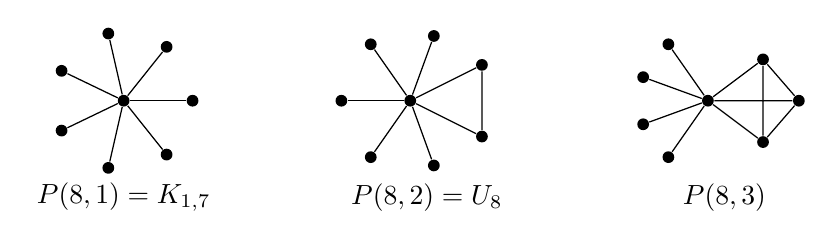
\begin{tikzpicture}[scale=.70,vertex/.style={circle,fill=black,inner sep=1.5pt},line width=.45pt]
\begin{scope}
\node[vertex] (a) at (0,0) {};
\foreach \theta [count=\i] in {0,51.43,102.86,154.29,205.71,257.14,308.57}{
\node[vertex] (l\i) at (\theta:1.25) {};
\draw (a)--(l\i);}
\node at (0,-1.75) {$P(8,1)=K_{1,7}$};
\end{scope}
\begin{scope}[xshift=5.2cm]
\node[vertex] (a) at (0,0) {};
\foreach \theta [count=\i] in {70,125,180,235,290}{
\node[vertex] (l\i) at (\theta:1.25) {};
\draw (a)--(l\i);}
\node[vertex] (b) at (1.3,.65) {};
\node[vertex] (c) at (1.3,-.65) {};
\draw (a)--(b)--(c)--(a);
\node at (.3,-1.75) {$P(8,2)=U_8$};
\end{scope}
\begin{scope}[xshift=10.6cm]
\node[vertex] (a) at (0,0) {};
\node[vertex] (b) at (1,.75) {};
\node[vertex] (c) at (1.65,0) {};
\node[vertex] (d) at (1,-.75) {};
\draw (a)--(b)--(c)--(d)--(a)--(c) (b)--(d);
\foreach \theta [count=\i] in {125,160,200,235}{
\node[vertex] (l\i) at (\theta:1.25) {};
\draw (a)--(l\i);}
\node at (.3,-1.75) {$P(8,3)$};
\end{scope}
\end{tikzpicture}
\caption{The star and two other pineapple graphs appearing in the entropy bounds.}
\label{fig:extremal-graphs}
% Alt text: Three eight-vertex graphs. Left: a star with seven leaves. Centre: a triangle with five leaves attached to one triangle vertex. Right: a four-vertex clique with four leaves attached to one clique vertex.
\end{figure}



The proof combines Laplacian coefficient inequalities with an
integral representation of entropy. Csikv\'ari \cite{Csikvari2011}
proved that Kelmans transformations do not increase Laplacian
coefficients and established a reduction to threshold graphs.
Entropy formulas in terms of characteristic polynomials and symmetric
functions were studied by Fannes \cite{Fannes2014}, Jozsa and Mitchison
\cite{JozsaMitchison2015}, and Sra \cite{Sra2019}.
The change in the second Laplacian coefficient makes the determinant
comparison strict for every proper Kelmans transformation, and the
entropy integral then gives a strict reduction to threshold graphs.
It remains to minimize entropy within this class. At fixed trace,
strict convexity reduces the optimization over the parameters of the
nested neighbourhoods to vectors with at most one intermediate
constant block. An endpoint comparison removes that block, and two
monotonicity arguments identify the pineapple as the unique minimizer.
This optimization proves Theorem~\ref{thm:threshold}.

Threshold graphs also arise in related problems with prescribed order
and size. Gong, Zou, and Zhang \cite{GongZouZhang2021} studied
minimizers of individual Laplacian coefficients, and Zhang et al.\
\cite{Zhang2025} studied graphs that minimize all coefficients
simultaneously. Luo, Gong, and Tian \cite{LuoGongTian2024} determined
the minimum of $\sum_i\sqrt{\mu_i}$ among connected graphs with
prescribed order and size. Here the optimization within the threshold
class allows the number of edges, and hence the normalizing trace,
to vary; the constraints are the order and the clique number.

Sections~\ref{sec:threshold-reduction} and
\ref{sec:threshold-minimum} prove Theorem~\ref{thm:main}.
Section~\ref{sec:prescribed-parameters} establishes the bounds with
prescribed parameters. Section~\ref{sec:all-renyi} treats R\'enyi
entropy, the nontree and tree extrema, and the counterexamples.

In addition to the notation above, $d_G(v)$ denotes vertex degree,
$\omega(G)$ the clique number, and $\chi(G)$ the chromatic number.
$N_G(v)$ denotes the open neighbourhood of $v$, with the subscript
omitted when the graph is clear, and $e(G)=|E(G)|$ denotes the size.
We write $\Spec_+(L_G)$ for the multiset of positive Laplacian eigenvalues.
Isolated vertices count as connected components. The symbol $\sqcup$
denotes disjoint union and $\vee$ denotes the graph join.


\section{Reduction to threshold graphs}\label{sec:threshold-reduction}
\subsection{Entropy under Kelmans transformations}\label{subsec:determinant-comparison}
We first reduce the entropy problem to connected threshold graphs while
preserving the order and size. The analytic ingredient is an equal-trace
version of the log-determinant formulas of Fannes~\cite{Fannes2014}
and Jozsa and Mitchison~\cite{JozsaMitchison2015}.
We give a proof that also verifies convergence when zero eigenvalues
are present. For related coefficient monotonicity results, see
Sra~\cite[Theorem 2.3]{Sra2019}.

\begin{samepage}
\begin{lemma}\label{lem:integral}
Let $A,B$ be positive semidefinite matrices of the same order and trace.
Then
\begin{equation}\label{eq:logdet-integral}
 \tr(A\log A)-\tr(B\log B)
 =-\int_0^\infty\log\frac{\det(tI+A)}{\det(tI+B)}\,dt.
\end{equation}
\end{lemma}
\end{samepage}
\begin{proof}
For $x\ge0$, an antiderivative of $\log(t+x)$ is
$(t+x)\log(t+x)-(t+x)$, with the continuous convention at zero.
Apply this antiderivative to the eigenvalues of the two matrices and
subtract the resulting integrals from $0$ to $R$.
Since the traces agree, the lower endpoint contributes the negative
of the trace difference in~\eqref{eq:logdet-integral}.
At the upper endpoint, equality of the orders and traces cancels the terms of orders
$R\log R$, $R$, and $\log R$, leaving a quantity tending to zero.
The integrand is $O(t^{-2})$ at infinity; at zero it is at worst
$O(|\log t|)$. This also verifies convergence.
\end{proof}

A \emph{Kelmans transformation} on vertices $u,v$ replaces each edge $vw$ for
$w\in N(v)\setminus(N(u)\cup\{u\})$ by $uw$; all other edges remain.
It preserves the order and size. It is \emph{proper} if both exclusive
neighbour sets are nonempty. A nonproper transformation either leaves the
graph unchanged or gives an isomorphic graph by interchanging $u$ and $v$.
Csikv\'ari proved that these transformations do not increase any elementary
symmetric coefficient of the Laplacian spectrum~\cite[Theorem~8.1]{Csikvari2011}.
The second coefficient makes this comparison strict for proper transformations.

\begin{lemma}[Strict determinant comparison]\label{lem:kelmans-determinant}
Let $G'$ be obtained from a simple graph $G$ by a Kelmans transformation
with beneficiary $u$ and co-beneficiary $v$. Then, for every $t>0$,
\[
 \det(tI+L_G)\ge\det(tI+L_{G'}).
\]
The inequality is strict for every $t>0$ if both exclusive neighbour sets
$N_G(u)\setminus(N_G(v)\cup\{v\})$ and
$N_G(v)\setminus(N_G(u)\cup\{u\})$ are nonempty; otherwise equality
holds for every $t>0$.
\end{lemma}
\begin{proof}
Write $\det(tI+L_G)=\sum_{j=0}^n e_j(G)t^{n-j}$, where $e_j(G)$ is
the $j$th elementary symmetric function of the Laplacian eigenvalues.
Csikv\'ari's coefficient comparison gives $e_j(G)\ge e_j(G')$ for every $j$.
Let $A$ and $B$ be the two exclusive neighbour sets, and put
$\alpha=|A|$, $\beta=|B|$. Only the degrees of $u,v$ change, and
$\sum_w d_{G'}(w)^2-\sum_w d_G(w)^2=2\alpha\beta$.
Since $G$ and $G'$ have the same size $m$,
\[
 e_2(G)=\frac{(2m)^2-\tr L_G^2}{2}
       =2m^2-m-\frac12\sum_w d_G(w)^2.
\]
Thus $e_2(G)-e_2(G')=\alpha\beta$. If the transformation is proper,
its determinant difference is therefore
at least $\alpha\beta t^{n-2}>0$. Otherwise the graphs are isomorphic,
so their determinants agree.
\end{proof}


\subsection{Reduction to connected threshold graphs}\label{subsec:connected-threshold-reduction}
A threshold graph is obtained from a single vertex by successively adding
an isolated vertex or a vertex adjacent to all existing vertices. The next
lemma gives the connected reduction needed here.

\begin{lemma}[A component-preserving threshold reduction]
\label{lem:elementary-threshold-reduction}
Every connected simple graph can be transformed into a connected threshold
graph by a sequence of proper Kelmans transformations. The sequence can
be empty, and it is nonempty whenever the original graph is not threshold.
\end{lemma}
\begin{proof}
Csikv\'ari's reduction theorem~\cite[Theorem~2.6(b)]{Csikvari2011}
provides a sequence of Kelmans transformations whose terminal threshold
graph has the same number of components as the original graph.
Transformations that give isomorphic graphs can be omitted by
relabelling the vertices in subsequent steps.
Every remaining step is proper. A nonthreshold graph requires at least
one such step, since being threshold is invariant under isomorphism.
\end{proof}


\begin{proposition}\label{prop:threshold-reduction}
Every connected graph $G$ of order at least two has a connected threshold
graph $T$ with the same order and size such that $\Ent(T)\le\Ent(G)$. If $G$ is not a
threshold graph, $T$ can be chosen with strict inequality.
\end{proposition}
\begin{proof}
Put $P_G(t)=\det(tI+L_G)$. If $G'$ is a Kelmans transform of $G$,
Lemma~\ref{lem:kelmans-determinant} gives $P_{G'}(t)\le P_G(t)$ for $t>0$.
Since the Laplacian traces agree, Lemma~\ref{lem:integral} gives
\begin{equation}\label{eq:kelmans-entropy}
 2m\bigl(\Ent(G)-\Ent(G')\bigr)
 =\int_0^\infty\log\frac{P_G(t)}{P_{G'}(t)}\,dt\ge0,
\end{equation}
with strict inequality for every proper transformation.
Apply Lemma~\ref{lem:elementary-threshold-reduction}.
If $G$ is not threshold, the sequence contains a proper transformation,
so the entropy inequality is strict.
\end{proof}

\section{The minimum on threshold graphs}\label{sec:threshold-minimum}
The reduction in Section~\ref{sec:threshold-reduction} preserves the number
of edges. To compare the resulting threshold graph with the star, we now
allow the number of edges to vary. We first minimize over threshold
graphs of a fixed clique number, then compare the resulting pineapple graphs.

\subsection{Nested degrees and a local perturbation}\label{subsec:ordered-polytope}
Fix a construction of a connected threshold graph by isolated and
dominating vertices, starting with one isolated vertex. The final vertex
is dominating when the graph has at least two vertices. Let $r$ be
the number of dominating vertices, and put $q=r+1$ and $N=n-q$.
The dominating vertices together with the initial vertex form a maximum
clique, so $q$ is the clique number. The remaining $N$ vertices are
independent, with degrees $b_1,\ldots,b_N\in\{1,\ldots,r\}$.
Order the dominating vertices by their neighbourhoods in the independent
set, and put
$c_i=|\{j:b_j\ge i\}|$. Thus
\begin{equation}\label{eq:ordered-domain}
 N=c_1\ge c_2\ge\cdots\ge c_r\ge0.
\end{equation}
The nonzero Laplacian spectrum is
\begin{equation}\label{eq:threshold-spectrum}
 \{q+c_i:1\le i\le r\}\ \cup\ \{b_j:1\le j\le N\}.
\end{equation}
This spectrum formula follows by induction: adding an isolated vertex
adds a zero eigenvalue, while adding
a dominating vertex to a graph of order $p$ gives eigenvalues $0,p+1$
and $1+\mu_i$ for the old eigenvalues, with one occurrence of zero omitted.
Equivalently,
the spectrum consists of the degrees of the isolated-type vertices
other than the initial vertex, the degrees plus one of the dominating
vertices, and zero; see also~\cite[Section 10]{Csikvari2011}.

Let $f(t)=t\log t$, with $f(0)=0$, and let
$d_i=f(i)-f(i-1)$. The tail-count identity
$\sum_j f(b_j)=\sum_i c_i d_i$ turns \eqref{eq:entropy} into
\begin{equation}\label{eq:TF-general}
 T=rq+2\sum_{i=1}^r c_i,\qquad
 F=\sum_{i=1}^r\bigl(f(q+c_i)+d_i c_i\bigr),\qquad
 \Ent=\log T-F/T.
\end{equation}

\begin{lemma}\label{lem:polytope}
Fix $n,r$ with $N>0$, and fix the sum of the $c_i$ in
\eqref{eq:ordered-domain}. To obtain a lower bound for the entropy,
it suffices to consider real vectors of the form
\begin{equation}\label{eq:three-platform}
 (N^{(a)},x^{(b)},0^{(c)}),\qquad
 a\ge1,\quad a+b+c=r,\quad 0\le x\le N,
\end{equation}
where the block lengths are nonnegative integers. The middle block
can be absent.
\end{lemma}
\begin{proof}
Allow the $c_i$ to be real. The feasible set defined by the order
constraints and the prescribed sum is compact, so the entropy expression
attains its minimum. Since $T$ is fixed, this is equivalent to maximizing $F$.
Suppose a maximizer has two distinct constant blocks with values strictly
between $0$ and $N$, of lengths $p_1,p_2$. Add $\varepsilon/p_1$ to every
entry of the first block and subtract $\varepsilon/p_2$ from every entry
of the second. For sufficiently small $|\varepsilon|$, both signs preserve
the order constraints and the sum. Along this line $F$ is strictly convex,
since $f''(q+c_i)=1/(q+c_i)>0$, so it cannot have a maximum at
$\varepsilon=0$. Thus at most one intermediate block remains.
The first coordinate is $N$, so the resulting vector has the stated form.
\end{proof}

For the vector \eqref{eq:three-platform}, the numerator and trace are
\begin{align}\label{eq:three-platform-TF}
 T(x)&=rq+2aN+2bx,\notag\\
 F(x)&=a f(n)+b f(q+x)+c f(q)
            +(N-x)f(a)+xf(a+b).
\end{align}
For integer $x$ this corresponds to the nonzero spectral list
$n^{(a)},\allowbreak(q+x)^{(b)},\allowbreak q^{(c)},\allowbreak a^{(N-x)},\allowbreak(a+b)^{(x)}$.
The formulas remain well defined for real $x$.

\subsection{The three-block comparison}\label{subsec:three-level-comparison}


\begin{lemma}[Endpoint comparison for three-block vectors]\label{lem:three-level-endpoints}
Let $q\ge3$ and $r=q-1$. Let $a,b\ge1$ and $c\ge0$ be integers
such that $a+b+c=r$, and let $N>0$ be real. Put $f(t)=t\log t$ for $t>0$,
with $f(0)=0$. For $0\le x\le N$, define
\begin{align*}
 T(x)&=qr+2aN+2bx,\\
 F(x)&=a f(q+N)+b f(q+x)+c f(q)
       +N f(a)+x\bigl(f(a+b)-f(a)\bigr),\\
 E(x)&=\log T(x)-\frac{F(x)}{T(x)}.
\end{align*}
Then
\begin{equation}\label{eq:three-level-endpoints}
 E(x)\ge \min\{E(0),E(N)\}\qquad(0\le x\le N).
\end{equation}
The inequality is strict for $0<x<N$.
\end{lemma}

\begin{proof}
Set $k=a+b$, $\delta=(f(k)-f(a))/b$, and
\begin{equation}\label{eq:three-level-H}
 H(x)=2F(x)-T(x)\bigl(\log(q+x)+\delta-1\bigr).
\end{equation}
Differentiation gives
\begin{equation}\label{eq:three-level-derivatives}
 E'(x)=\frac{bH(x)}{T(x)^2},\qquad
 H'(x)=4b-\frac{T(x)}{q+x}.
\end{equation}
We prove that $H(x)>0$ whenever $H'(x)\ge0$. It then follows that every
interior critical point of $E$ satisfies
$E''(x)=bH'(x)/T(x)^2<0$. Thus $E$ has no interior local minimum, which
implies the asserted strict endpoint comparison.

Fix $x$ with $H'(x)\ge0$, write $y=q+x$, and introduce
\[
 W=\frac{a(q+N)}{qk},\qquad
 \xi=\frac{ay}{qk},\qquad
 \eta=\frac{by}{qk},\qquad
 d=\frac{r}{2k},\qquad
 \rho=\frac{W+d-1}{\eta}.
\]
Then $W\ge\xi>0$, $\eta>0$, $\xi+\eta=y/q\ge1$, and $d\ge1/2$.
Moreover,
\[
 \frac{T(x)}{2qk}=(1+\rho)\eta=W+\eta+d-1\ge d,
 \qquad H'(x)=2b(1-\rho),
\]
so $\rho\le1$. Direct substitution gives
\begin{equation}\label{eq:three-level-identity}
 \frac{H(x)}{2qk}
 =f(W)+\rho\bigl(f(\xi)-f(\xi+\eta)\bigr)
       +d\log(q/k)+(1+\rho)\eta.
\end{equation}
Since $\xi+\eta\ge1$ and $0<\xi<\xi+\eta$, we have
$f(\xi)<f(\xi+\eta)$. If $\rho\le0$, then $f(W)\ge-1/e$,
$\log(q/k)>0$, and $(1+\rho)\eta\ge1/2$, so the right-hand side of
\eqref{eq:three-level-identity} is at least $1/2-1/e>0$.

Suppose $0<\rho\le1$. By convexity of $f$ and $W\ge\xi$,
\[
 f(\xi)-f(\xi+\eta)\ge f(W)-f(W+\eta).
\]
Also $q/k>r/k=2d$. Therefore
\[
 \frac{H(x)}{2qk}
 \ge(1+\rho)f(W)-\rho f(W+\eta)
          +d\log(2d)+(1+\rho)\eta.
\]
Set $Y=W+\eta\ge1$. Since
$(1+\rho)W+d=1+\rho Y$ and
$(1+\rho)\eta=Y+d-1\ge Y-1/2$, the log-sum inequality gives
\begin{align*}
 \frac{H(x)}{2qk}
 &\ge (1+\rho Y)\log\frac{1+\rho Y}{\rho+3/2}
       -\rho Y\log Y+Y-\frac12\\
 &=f(1+\rho Y)-f(\rho Y)-\log(\rho+3/2)
   +Y\left(1-\rho\log\left(1+\frac{3}{2\rho}\right)\right)
   -\frac12.
\end{align*}
The coefficient of $Y$ is positive, since concavity of the logarithm gives
$\rho\log(1+3/(2\rho))\le\log(5/2)<1$.
Moreover, convexity of $f$ implies
$f(1+\rho Y)-f(\rho Y)\ge f(1+\rho)-f(\rho)$.
Thus both terms depending on $Y$ are minimized at $Y=1$, and
\[
 \frac{H(x)}{2qk}
 \ge\frac12-(1+\rho)\log\left(1+\frac{1}{2(1+\rho)}\right)>0
\]
by $\log(1+t)<t$. Hence $H(x)>0$, as required.
\end{proof}

\begin{remark}
At $x=0$ the middle block merges with the zero block, whereas at $x=N$
it merges with the block of entries equal to $N$. If $N=0$, $b=0$, or
$q=2$, there is no genuine three-block comparison to make.
\end{remark}

\subsection{Two monotonicity comparisons}\label{subsec:two-monotonicity-comparisons}

\begin{lemma}[Monotonicity in the number of largest eigenvalues]
\label{lem:two-level-a}
Let $n$ and $r$ be integers with $1\le r\le n-1$, and put
$q=r+1$ and $N=n-q$. For $1\le a\le r$, define
\begin{align*}
 T(a)&=qr+2Na,\\
 F(a)&=an\log n+(r-a)q\log q+Na\log a,\\
 \mathcal S_{n,r}(a)&=\log T(a)-\frac{F(a)}{T(a)}.
\end{align*}
If $N>0$ and $r>1$, then $\mathcal S_{n,r}(a)$ is strictly increasing
on $[1,r]$. If $N=0$, it is the constant $\log(n-1)$.
In particular, for integer $a$, the entropy obtained by normalizing
the positive eigenvalues
\[
 n^{(a)},\qquad q^{(r-a)},\qquad a^{(N)}
\]
is at least $\mathcal S_{n,r}(1)$.
\end{lemma}

\begin{proof}
The assertion is immediate when $N=0$. For $N>0$, put $t=N/q>0$,
$\lambda=a/r\in(0,1]$, and $J(t)=(1+t)\log(1+t)/t$.
Differentiation gives
\[
 \frac{T(a)^2}{Nqr}\mathcal S'_{n,r}(a)
 =2t\lambda-\log\lambda+\log(q/r)+1-J(t).
\]
Since $J(t)<\log(1+t)+1$ and $\lambda(1+t)\le1+\lambda t$, the right
side is greater than
\[
 2\lambda t-\log(1+\lambda t)+\log(q/r)
 >\lambda t+\log(q/r)>0.
\]
This proves the claimed strict increase.
\end{proof}

\begin{lemma}[Monotonicity of the pineapple spectral entropy]
\label{lem:pineapple-r}
Fix an integer $n\ge2$. For real $1\le r\le n-1$, put
\begin{align*}
 T(r)&=2n-2+r(r-1),\\
 F(r)&=n\log n+(r^2-1)\log(r+1),\\
 \mathcal P_n(r)&=\log T(r)-\frac{F(r)}{T(r)}.
\end{align*}
If $n>2$, the function $\mathcal P_n$ is strictly increasing. Consequently
\[
 \mathcal P_n(r)\ge\mathcal P_n(1)
 =\log(2n-2)-\frac{n\log n}{2n-2},
\]
with equality only at $r=1$.
For integer $r$, $\mathcal P_n(r)$ is the entropy obtained by normalizing
the positive eigenvalues
$n,(r+1)^{(r-1)},1^{(n-r-1)}$.
\end{lemma}

\begin{proof}
There is nothing to prove when $n=2$. For $n>2$, write $q=r+1$ and
$t=(n-q)/q\ge0$. Direct differentiation and substitution give
\begin{align*}
 \frac{T(r)^2}{q}\mathcal P_n'(r)
 ={}&(2r-1)(1+t)\log\frac{1+t}{q}\\
    &+2(r-\log q)t+(r-1)\log q+r^2.
\end{align*}
The inequality $z\log(z/q)\ge-q/e$ for $z>0$, together with
$\log(r+1)<r$ and $(2r-1)(r+1)\le9r^2/4$, therefore yields
\[
 \frac{T(r)^2}{q}\mathcal P_n'(r)
 \ge r^2\left(1-\frac9{4e}\right)>0.
\]
Here the quadratic bound is equivalent to $(r-2)^2\ge0$.
\end{proof}


\subsection{Proof of the extremal theorems}\label{subsec:completion}
\begin{proof}[Proof of Theorem~\ref{thm:threshold}]
If $N=0$, the graph is $K_n=\Pine(n,n-1)$. If $r=1$, it is the star.
Suppose $N>0$ and $r\ge2$. Use Lemma~\ref{lem:polytope} at the trace
of the given graph. If a minimizing vector has an intermediate block,
Lemma~\ref{lem:three-level-endpoints} shows that its entropy is at least
the smaller endpoint value. Each endpoint vector has the form
$(N^{(a)},0^{(r-a)})$ for some integer $a$,
with spectral list $n^{(a)},(r+1)^{(r-a)},a^{(N)}$.
By Lemma~\ref{lem:two-level-a}, the smallest entropy among these vectors
occurs at $a=1$, which corresponds to $\Pine(n,r)$.

The preceding argument establishes the bound throughout the real ordered
domain. For uniqueness, the inequality is strict for every two-block
vector with $a>1$. A vector with a genuine intermediate block has entropy
strictly greater than the smaller endpoint value. If the original vector
has two distinct intermediate blocks, the perturbation in
Lemma~\ref{lem:polytope} strictly lowers its entropy in one direction.
It therefore cannot attain the lower bound.
Thus equality can only occur for $(N,0,\ldots,0)$, which describes $\Pine(n,r)$.
Finally, Lemma~\ref{lem:pineapple-r} gives the strict increase with $r$.
\end{proof}

\begin{proof}[Proof of Theorem~\ref{thm:main}]
By Proposition~\ref{prop:threshold-reduction}, choose a connected
threshold graph $T$ of the same order and size with
$\Ent(G)\ge\Ent(T)$. If $r+1$ is the clique number of $T$, then
Theorem~\ref{thm:threshold} and Lemma~\ref{lem:pineapple-r} give
\[
 \Ent(G)\ge\Ent(T)\ge\Ent(\Pine(n,r))
 \ge\Ent(\Pine(n,1))=\Ent(K_{1,n-1}).
\]
If $G$ is not threshold, the first inequality is strict. If it is
threshold and is not the star, then $r\ge2$, so the final comparison is
strict. This proves both the bound and its equality characterization.
\end{proof}


\section{Sharp bounds with prescribed graph parameters}
\label{sec:prescribed-parameters}

We now sharpen the star bound by prescribing the clique or chromatic
number. The results also apply to disconnected graphs, with the number
of components expressed through the Laplacian rank. Equality is attained
by a pineapple graph together with isolated vertices.

The next observation follows from Csikv\'ari's stronger theorem that
Kelmans transformations do not decrease the number of cliques of any
given size \cite[Theorem 5.10]{Csikvari2011}. We include a short proof.

\begin{lemma}[Clique number under a Kelmans transformation]
\label{lem:kelmans-clique}
If $G'$ is obtained from a simple graph $G$ by a Kelmans transformation,
then $\omega(G')\ge\omega(G)$.
\end{lemma}
\begin{proof}
Let $u$ be the beneficiary and $v$ the other vertex. A clique $Q$ of
$G$ survives if $v\notin Q$ or if $u,v\in Q$; in the latter case its
other vertices are common neighbours. Otherwise,
$(Q\setminus\{v\})\cup\{u\}$ is a clique of $G'$, since $u$ is
adjacent in $G'$ to every former neighbour of $v$ other than $u$.
\end{proof}

\begin{theorem}[Rank and clique number]
\label{thm:clique-rank}
Let $G$ be a simple graph with at least one edge, $n$ vertices, and $k$
connected components, including isolated vertices. Set
$s=n-k+1=\operatorname{rank}L_G+1$ and $r=\omega(G)-1$.
Then $1\le r\le s-1$ and
\begin{equation}\label{eq:clique-rank}
 \begin{aligned}
 \Ent(G)&\ge\Ent(\Pine(s,r))\\
 &=\log\bigl(2s-2+r(r-1)\bigr)
 -\frac{s\log s+(r^2-1)\log(r+1)}{2s-2+r(r-1)}.
 \end{aligned}
\end{equation}
Equality holds if and only if
$G\cong\Pine(s,r)\,\sqcup\,(k-1)K_1$.
\end{theorem}
\begin{proof}
The kernel of $L_G$ consists of the vectors that are constant on each
component, so $\operatorname{rank}L_G=n-k$. Every component has at most
$s$ vertices, which gives $1\le r\le s-1$.

If two components contain edges, choose vertices $u,v$ of positive
degree in different components and apply the Kelmans transformation
with beneficiary $u$. Their neighbourhoods are disjoint, so the
transformation transfers all edges incident with $v$ to $u$ and leaves
$v$ isolated. Every component remaining after $v$ is deleted from its
original component contains a former neighbour of $v$ and is therefore
joined to $u$. The two original
components are replaced by one component containing edges and one
isolated vertex. The step is proper and preserves the number of
components.

Repeat until only one component contains edges. It has $s$ vertices.
Apply Proposition~\ref{prop:threshold-reduction} to that component,
leaving the isolated vertices fixed. This produces a graph
$T=H\sqcup(k-1)K_1$, where $H$ is a connected threshold graph of
order $s$. The transformations preserve order, size, and the number of
components. Lemma~\ref{lem:kelmans-determinant}
and \eqref{eq:kelmans-entropy} also apply to disconnected graphs,
so $\Ent(G)\ge\Ent(T)=\Ent(H)$, strictly if any step is proper.

Put $r'=\omega(H)-1$. Lemma~\ref{lem:kelmans-clique} gives $r'\ge r$.
Theorem~\ref{thm:threshold} and the strict increase of the pineapple
entropy in its clique parameter imply
\[
 \Ent(G)\ge\Ent(H)\ge\Ent(\Pine(s,r'))
 \ge\Ent(\Pine(s,r)).
\]
The positive eigenvalues of $\Pine(s,r)$ are
$s,(r+1)^{(r-1)},1^{(s-r-1)}$, which gives
\eqref{eq:clique-rank}. If equality holds, no step is proper, so
$G\cong H\sqcup(k-1)K_1$. Also $r'=r$, and
Theorem~\ref{thm:threshold} gives
$H\cong\Pine(s,r)$. Hence $G\cong\Pine(s,r)\sqcup(k-1)K_1$.
Conversely, this graph has the prescribed parameters and attains the
bound, since isolated vertices do not change the entropy.
\end{proof}

\begin{corollary}[Prescribed clique number]
\label{cor:prescribed-clique}
For $n\ge2$ and $1\le r\le n-1$, the graph $\Pine(n,r)$ uniquely
minimizes von Neumann entropy among connected graphs of order $n$ and
clique number $r+1$. It is also the unique minimizer among connected
graphs of order $n$ containing a copy of $K_{r+1}$.
\end{corollary}
\begin{proof}
Use Theorem~\ref{thm:clique-rank} with $k=1$, together with the strict
increase of $\Ent(\Pine(n,t))$ in $t$.
\end{proof}

\subsection{Prescribed chromatic number}

Clique number is nondecreasing under every Kelmans transformation,
but chromatic number need not be. To retain a chromatic lower bound
while preserving components, we first restrict the transformation to
nonadjacent vertices with a common neighbour.

\begin{lemma}[A reduction preserving a chromatic lower bound]
\label{lem:chromatic-reduction}
For every simple graph $G$ with at least one edge, there is a simple graph
$H$ of the same order, size, and number of components such that
\[
 \Ent(H)\le\Ent(G),\qquad
 \chi(H)\ge\chi(G),\qquad \chi(H)=\omega(H).
\]
Moreover, the construction below either leaves $G$ unchanged or gives
$\Ent(H)<\Ent(G)$.
\end{lemma}
\begin{proof}
Apply a proper Kelmans transformation only to nonadjacent vertices
$u,v$ having a common neighbour. With $u$ as beneficiary, their new
neighbourhoods are
$N_{G'}(u)=N_G(u)\cup N_G(v)$ and
$N_{G'}(v)=N_G(u)\cap N_G(v)$.
Any proper colouring of $G'$ gives a colouring of $G$ using at most the
same number of colours: give $v$ the colour of $u$ and retain all other
colours. This is valid because $uv\notin E(G)$ and every neighbour of
$v$ in $G$ is a neighbour of $u$ in $G'$. Hence $\chi(G')\ge\chi(G)$.

If $w$ is a common neighbour of $u,v$, then $uw$ and $vw$ remain edges.
Every removed edge $vx$ can be replaced by the path $v,w,u,x$ in $G'$.
Thus the transformation preserves the components. By
Lemma~\ref{lem:kelmans-determinant} and \eqref{eq:kelmans-entropy}, it
strictly decreases entropy. It also strictly increases the integer
$\sum_z d(z)^2$, so the process terminates.

In the resulting graph $H$, nonadjacent vertices with a common neighbour
have comparable open neighbourhoods. This property is inherited by
induced subgraphs. Let $J$ be an induced subgraph with a component that
is not complete, and choose an induced path $u,w,v$ in that component.
Interchange $u,v$ if necessary so that $N_J(u)\subseteq N_J(v)$.
Every colouring of $J-u$ extends to $J$ by giving $u$ the colour of $v$.
Likewise, replacing $u$ by $v$ in any clique containing $u$ gives
a clique of $J-u$ of the same order.
Therefore $\chi(J)=\chi(J-u)$ and $\omega(J)=\omega(J-u)$.
Repeated deletion reduces $J$ to a disjoint union of cliques, where
these parameters agree. Taking $J=H$ gives $\chi(H)=\omega(H)$;
the argument for every induced subgraph also shows that $H$ is perfect.
The strictness assertion follows from the strict decrease at each step.
\end{proof}

\begin{theorem}[Rank and chromatic number]
\label{thm:chromatic-rank}
Let $G$ be a simple graph with at least one edge, $n$ vertices, and $k$
connected components. Set $s=n-k+1=\operatorname{rank}L_G+1$ and
$r=\chi(G)-1$. Then $1\le r\le s-1$ and
\begin{equation}\label{eq:chromatic-rank}
 \Ent(G)\ge\Ent(\Pine(s,r)),
\end{equation}
where the right-hand side is given in \eqref{eq:clique-rank}.
Equality holds if and only if
$G\cong\Pine(s,r)\sqcup(k-1)K_1$.
In particular, $\Pine(n,r)$ uniquely minimizes entropy among connected
graphs of order $n$ and chromatic number $r+1$.
\end{theorem}
\begin{proof}
Every component has at most $s$ vertices, so $2\le\chi(G)\le s$.
Let $H$ be given by Lemma~\ref{lem:chromatic-reduction}. Since its
number of components is unchanged, Theorem~\ref{thm:clique-rank}
gives
\[
 \Ent(G)\ge\Ent(H)
 \ge\Ent\bigl(\Pine(s,\omega(H)-1)\bigr)
 =\Ent\bigl(\Pine(s,\chi(H)-1)\bigr)
 \ge\Ent(\Pine(s,r)).
\]
The last inequality uses the monotonicity of pineapple entropy.
If equality holds, the reduction performs no step, so $H=G$.
Strict monotonicity and equality in Theorem~\ref{thm:clique-rank}
then give $G\cong\Pine(s,r)\sqcup(k-1)K_1$.
The converse follows directly from the spectrum and chromatic number
of this graph.
\end{proof}

\begin{remark}
The restriction to nonadjacent vertices in
Lemma~\ref{lem:chromatic-reduction} is necessary. On the cycle
$0,1,2,3,4,0$, the Kelmans transformation with beneficiary $0$ and other
vertex $1$ replaces $12$ by $02$. The resulting graph is a $4$-cycle
with a pendant vertex and has chromatic number $2$, whereas the
original graph has chromatic number $3$.
\end{remark}

\section{R\'enyi entropies of order at least one}
\label{sec:all-renyi}

We now prove Conjecture~\ref{conj:star-renyi}, stated as
Conjecture 3.3 in~\cite{Dairyko2017}, using Theorem~\ref{thm:main}.
The uncapped inequality in Lemma~\ref{lem:shannon-renyi-transfer}
is a consequence of the fixed-alphabet entropy bounds of
Harremo\"es~\cite[Theorem 3]{Harremoes2009} and Sakai--Iwata
\cite[extended version, Theorem 1 and Corollary 1]{SakaiIwata2016}.
We include a direct proof that records the equality cases and the
endpoint $\alpha=\infty$, and then establish the capped comparison
needed for nontrees.

For a probability vector $p=(p_1,\ldots,p_k)\in[0,1]^k$ with
$\sum_i p_i=1$, allowing zero coordinates, write
$H(p)=-\sum_i p_i\log p_i$, $R_\alpha(p)=\sum_i p_i^\alpha$,
and $H_\alpha(p)=\log R_\alpha(p)/(1-\alpha)$ for
$\alpha>0$, $\alpha\ne1$. We use $0\log0=0$, put
$H_1(p)=H(p)$, and set $H_\infty(p)=-\log\max_i p_i$.

\begin{lemma}[An entropy-preserving variation]
\label{lem:entropy-preserving-variation}
Let $x_0\ge y_0>z_0\ge0$. There are triples $(x,y,z)$ arbitrarily close
to $(x_0,y_0,z_0)$ with $x>x_0$, $y<y_0$, $z>z_0$ and $x>y>z>0$,
having the same sum and the same value of
$x\log x+y\log y+z\log z$ as the original triple, such that
\[
 x^\alpha+y^\alpha+z^\alpha
 >x_0^\alpha+y_0^\alpha+z_0^\alpha
 \qquad(\alpha>1).
\]
\end{lemma}
\begin{proof}
Write $g(t)=t\log t$, $g(0)=0$, and $s=x_0+y_0+z_0$. For
$z>z_0$ close to $z_0$, put
\[
 F_z(x)=g(x)+g(s-z-x)+g(z)
        -g(x_0)-g(y_0)-g(z_0).
\]
A small transfer from $y_0$ to $z_0$ gives $F_z(x_0)<0$.
Choose a small $\varepsilon>0$ with $y_0-\varepsilon>z_0$.
Strict convexity gives $F_{z_0}(x_0+\varepsilon)>0$, so this sign
persists for $z$ sufficiently close to $z_0$. Between these endpoints,
with $y=s-z-x$, one has $x>y>z>0$ and
$\partial F_z/\partial x=\log(x/y)>0$. The intermediate value theorem
therefore gives a unique root $x=x(z)>x_0$, with $y(z)<y_0$.
The root tends to $x_0$ as $z\downarrow z_0$, including when
$x_0=y_0$ or $z_0=0$.

Along this branch,
\[
 \frac{dx}{dz}=\frac{\log(y/z)}{\log(x/y)},\qquad
 \frac{dy}{dz}=-\frac{\log(x/z)}{\log(x/y)}.
\]
For $\beta=\alpha-1>0$, it follows that
\[
 \frac1\alpha\frac{d}{dz}(x^\alpha+y^\alpha+z^\alpha)
 =\log(y/z)\left[
 \frac{x^\beta-y^\beta}{\log x-\log y}
 -\frac{y^\beta-z^\beta}{\log y-\log z}\right]>0,
\]
by strict convexity of $u\mapsto e^{\beta u}$. Continuity at the
initial triple proves the assertion, also when it has a zero coordinate.
\end{proof}

\begin{lemma}[Shannon-to-R\'enyi comparison]
\label{lem:shannon-renyi-transfer}
Let $k\ge2$, $1/k<a<1$, $b=(1-a)/(k-1)$, and
$v=(a,b,\ldots,b)$. If a probability vector $p$ with $k$ coordinates satisfies
$H(p)\ge H(v)$, then
\[
 H_\alpha(p)\ge H_\alpha(v)\qquad(1<\alpha\le\infty).
\]
For each such $\alpha$, equality holds if and only if $p$ is a
permutation of $v$.
\end{lemma}
\begin{proof}
For $x=\max_i p_i$, concavity gives
\[
 H(p)\le J_k(x):=-x\log x-(1-x)\log\frac{1-x}{k-1}.
\]
The function $J_k$ strictly decreases on $[1/k,1]$. Thus
$H(p)\ge J_k(a)$ implies $x\le a$, with $x=a$ only when all other
coordinates equal $b$. This proves the infinite-order assertion.

Fix $\alpha>1$, put $h=H(v)$, and maximize $R_\alpha$ on the
compact set of probability vectors with entropy at least $h$.
At a maximizer $q$, the entropy constraint is active: otherwise a
small movement of the sorted vector towards $(1,0,\ldots,0)$
strictly increases the power sum by strict Schur convexity while
remaining feasible.
Since $h>0$, a maximizer with a zero coordinate would have at least
two positive coordinates. Lemma~\ref{lem:entropy-preserving-variation}
applied to these and a zero coordinate gives a contradiction.
Hence $q$ is positive. The same lemma shows that at most one
coordinate exceeds the minimum: applying it to two such coordinates
and a smallest coordinate would strictly increase the power sum while
preserving the entropy. Since $h<\log k$, there is exactly
one larger coordinate. Thus $q=(x,(1-x)/(k-1),\ldots,(1-x)/(k-1))$
up to permutation, and $J_k(x)=J_k(a)$ forces $x=a$.
This characterizes every maximizer and proves the finite-order
inequality and its equality case.
\end{proof}

\begin{corollary}[Star minimality for all orders $\alpha\ge1$]
\label{cor:all-renyi-star}
Let $G$ be a connected simple graph on $n\ge2$ vertices. For every
$1\le\alpha\le\infty$, we have
\[
 H_\alpha(G)\ge H_\alpha(K_{1,n-1})=
 \begin{cases}
 \displaystyle\log(2n-2)-\frac{n\log n}{2n-2},&\alpha=1,\\[6pt]
 \displaystyle\frac{1}{1-\alpha}
       \log\frac{n^\alpha+n-2}{(2n-2)^\alpha},&1<\alpha<\infty,\\[6pt]
 \displaystyle\log\frac{2n-2}{n},&\alpha=\infty.
 \end{cases}
\]
For each order, equality holds if and only if $G\cong K_{1,n-1}$.
\end{corollary}

\begin{proof}
For $n=2$, the only connected simple graph is $K_2$, and its positive
normalized Laplacian spectrum is $(1)$, giving all assertions.
For $n\ge3$, connectedness gives exactly $k=n-1$ positive normalized
Laplacian eigenvalues. Regard them as a probability vector $p$.
The corresponding star vector is
\[
 v=\left(\frac{n}{2n-2},
         \underbrace{\frac1{2n-2},\ldots,\frac1{2n-2}}_{n-2}\right).
\]
Theorem~\ref{thm:main} gives $H(p)\ge H(v)$, strictly unless $G$ is
the star. Apply Lemma~\ref{lem:shannon-renyi-transfer}. Its equality
condition implies $H(p)=H(v)$, so the equality characterization in
Theorem~\ref{thm:main} gives the claimed equality case for every order.
\end{proof}

For comparison, the conclusion for finite $\alpha>2$ can also be
deduced without Theorem~\ref{thm:main}. Put $k=n-1$ and
$v_t=(t,(1-t)/(k-1),\ldots,(1-t)/(k-1))$, where $1/k\le t\le1$.
For $n\ge3$, choose $t$ with $H_\alpha(v_t)=H_\alpha(p)$.
Harremo\"es' theorem \cite[Theorem 3]{Harremoes2009} gives
$H_2(p)\le H_2(v_t)$. For a nonstar, the strict bound in
\cite[Theorem 3.8]{Dairyko2017} implies
$H_2(v_t)>H_2(v_{n/(2n-2)})$.
Since each $H_\beta(v_t)$ strictly decreases with $t$ for $\beta>0$,
we obtain $t<n/(2n-2)$ and hence the strict $\alpha$-entropy bound.
The case $n=2$ is immediate.

\begin{remark}[Quantitative transfer]
Under the hypotheses of Lemma~\ref{lem:shannon-renyi-transfer}, fix
$\alpha>1$. For $f(t)=t^\alpha$ and $g(t)=t\log t$, write
\[
 D_\varphi(t,b)=\varphi(t)-\varphi(b)-\varphi'(b)(t-b),\qquad
 A=\frac{D_f(a,b)}{D_g(a,b)}>0.
\]
The ratio $D_f(t,b)/D_g(t,b)$, continuously extended at $t=b$,
is strictly increasing. Indeed, the ratio of the derivatives of the
numerator and denominator is
\[
 \frac{\partial_tD_f(t,b)}{\partial_tD_g(t,b)}
 =\alpha(\alpha-1)\int_0^1
 b^{(\alpha-1)(1-s)}t^{(\alpha-1)s}\,ds,
\]
which strictly increases with $t$. The original ratio is a weighted
average of this expression between $b$ and $t$, with positive
weight $|\log(u/b)|$ in the integration variable $u$; differentiating
the quotient proves monotonicity on both sides of $b$.
The ratio extends continuously to $t=0$. Consequently
\begin{equation}\label{eq:renyi-scalar-majorant}
 D_f(t,b)\le A D_g(t,b)\qquad(0\le t\le a),
\end{equation}
with equality exactly at $t=b,a$. Since $\max_i p_i\le a$, summing
and using the equal total masses gives
\[
 R_\alpha(v)-R_\alpha(p)\ge A\bigl(H(p)-H(v)\bigr).
\]
The inequality $-\log t\ge1-t$ therefore yields
\[
 H_\alpha(p)-H_\alpha(v)
 \ge\frac{A}{(\alpha-1)R_\alpha(v)}
       \bigl(H(p)-H(v)\bigr).
\]
For the star vector, with $n\ge3$, this coefficient is
\[
 \frac{2(n-1)\,[n^\alpha-1-\alpha(n-1)]}
 {(\alpha-1)(n\log n-n+1)(n^\alpha+n-2)},
\]
and tends to $1$ as $\alpha\downarrow1$. At infinite order,
\[
 H_\infty(p)-H_\infty(v)
 \ge\frac{H(p)-H(v)}{a\log(a/b)}.
\]
Indeed, with $x=\max_i p_i$, the bound by $J_k$ gives
$H(p)-H(v)\le J_k(x)-J_k(a)\le(a-x)\log(a/b)$, while
$\log(a/x)\ge(a-x)/a$.
\end{remark}

\begin{corollary}[The rank version for all orders]
\label{cor:renyi-rank}
Let $G$ be a simple graph with at least one edge and
$d=\operatorname{rank}L_G$. For every $1\le\alpha\le\infty$,
\[
 H_\alpha(G)\ge H_\alpha(K_{1,d}),
\]
with equality exactly when $G$ is $K_{1,d}$ together with isolated vertices.
For $1<\alpha<\infty$, the right-hand side is
\[
 \frac1{1-\alpha}\log\frac{(d+1)^\alpha+d-1}{(2d)^\alpha}.
\]
\end{corollary}
\begin{proof}
For $d=1$, the graph is $K_2$ together with isolated vertices.
For $d\ge2$, Theorem~\ref{thm:clique-rank} and
Lemma~\ref{lem:pineapple-r} give the claimed von Neumann bound and its
unique equality case. Apply Lemma~\ref{lem:shannon-renyi-transfer} to
the $d$ positive normalized eigenvalues and the star vector of that length.
The equality case in the lemma forces equality in the von Neumann bound.
\end{proof}

\subsection{The sharp bound for connected nontrees}

The extremal form in the following comparison is related to the
boundary description for three R\'enyi entropies in
\cite[Section 4]{Harremoes2009}. We give a direct proof for the cap
$1/2$, including the inequality constraints and the equality case
needed for nontrees.

\begin{lemma}[A capped Shannon-to-R\'enyi comparison]\label{lem:capped-transfer}
Let $k\ge3$ and let $v=(1/2,a,b,\ldots,b)$ be a probability vector,
where $a>b>0$. If a probability vector $p$ with $k$ coordinates satisfies
$\max_i p_i\le1/2$ and $H(p)\ge H(v)$, then, for every finite
$\alpha>1$,
\[
 R_\alpha(p)\le R_\alpha(v),\qquad
 H_\alpha(p)\ge H_\alpha(v).
\]
Equality holds if and only if $p$ is a permutation of $v$.
\end{lemma}
\begin{proof}
Put $h=H(v)$. The positive, nonuniform tail gives
\[
 \log2<h<J_k(1/2).
\]
Fix $\alpha>1$ and maximize $R_\alpha$ on the compact feasible set.
At a maximizer $q$ one has $H(q)=h$: if the inequality were strict,
a small movement of the sorted vector towards $(1/2,1/2,0,\ldots,0)$
would strictly increase the power sum and remain feasible. This
follows from strict Schur convexity, since that vector majorizes
every probability vector with coordinates at most $1/2$.

Every feasible vector has at least two coordinates strictly between
$0$ and $1/2$. If $q$ had a zero coordinate, apply
Lemma~\ref{lem:entropy-preserving-variation} to two such interior
coordinates and that zero. A sufficiently small variation still
has all coordinates at most $1/2$, contradicting maximality.
If all coordinates were below $1/2$, the same variation would imply
that the maximizer is either uniform or has one coordinate larger
than the others, all of which are equal.
The uniform vector has entropy $\log k>h$; in the other case the
entropy is at least $J_k(1/2)>h$. Both contradict $H(q)=h$.
Consequently exactly one coordinate equals $1/2$.

Write $q=(1/2,r_1/2,\ldots,r_{k-1}/2)$ and
$s=(2a,2b,\ldots,2b)$. Then $H(r)=H(s)$, and
Lemma~\ref{lem:shannon-renyi-transfer} gives
\[
 R_\alpha(q)=2^{-\alpha}(1+R_\alpha(r))
 \le2^{-\alpha}(1+R_\alpha(s))=R_\alpha(v),
\]
with equality only when $r$ is a permutation of $s$.
This proves the assertion and characterizes all maximizers.
\end{proof}

\begin{corollary}[All finite orders for connected nontrees]
\label{cor:nontree-all-renyi}
Let $G$ be a connected simple nontree on $n\ge3$ vertices, and let
$U_n$ be the triangle with $n-3$ leaves attached to one triangle
vertex. For every finite $1\le\alpha<\infty$,
\[
 H_\alpha(G)\ge H_\alpha(U_n),
\]
with equality if and only if $G\cong U_n$. For $\alpha>1$ the
bound is explicitly
\[
 H_\alpha(G)\ge\frac1{1-\alpha}
 \log\frac{n^\alpha+3^\alpha+n-3}{(2n)^\alpha}.
\]
\end{corollary}
\begin{proof}
We first prove the assertion for $\alpha=1$.
Since $G$ has at least $n$ edges,
Proposition~\ref{prop:threshold-reduction} gives a connected threshold
graph $T$ of the same order and size with $\Ent(G)\ge\Ent(T)$,
strictly if $G$ is not threshold; otherwise take $T=G$.
Write $r+1=\omega(T)$. A connected threshold graph with clique
number two is a star, so the edge count forces $r\ge2$.
Theorem~\ref{thm:threshold} and Lemma~\ref{lem:pineapple-r} give
\[
 \Ent(G)\ge\Ent(T)\ge\Ent(\Pine(n,r))
 \ge\Ent(\Pine(n,2))=\Ent(U_n).
\]
The equality cases force $G\cong U_n$. Its positive spectrum
$(n,3,1^{(n-3)})$ gives
\begin{equation}\label{eq:nontree-minimum-value}
 \Ent(U_n)=\log(2n)-\frac{n\log n+3\log3}{2n}.
\end{equation}

For $n=3$, the only connected nontree is $K_3=U_3$, so all orders
are immediate. Let $n\ge4$ and $\alpha>1$, and let $p$ be the vector
of positive normalized Laplacian eigenvalues of $G$. Since
$e(G)\ge n$ and $\mu_{\max}(G)\le n$, we have $\max_i p_i\le1/2$.
The preceding argument gives $H(p)\ge\Ent(U_n)$, whose probability
vector is $(1/2,3/(2n),1/(2n),\ldots,1/(2n))$.
Lemma~\ref{lem:capped-transfer} proves the required inequality.
Its equality case forces $\Ent(G)=\Ent(U_n)$, and the equality
case already proved at order one gives $G\cong U_n$.
\end{proof}

Li, Chen, and Yang \cite{LiChenYang2015} computed the spectrum of
$U_n$ and proved that adding one edge between leaves of a star
increases its von Neumann entropy. For unicyclic graphs, the
coefficient theorem of Stevanovi\'c and Ili\'c
\cite[Theorem 1.3]{StevanovicIlic2009}, together with
Lemma~\ref{lem:renyi-coefficient-order} below, already gives the
corresponding entropy minimum for $0<\alpha\le2$. The result above
compares all connected nontrees, allowing their Laplacian traces to vary.

The order-two nontree bound is also a consequence of earlier results.
The unicyclic case follows from the coefficient comparison just cited.
If $m\ge n+1$, de Caen's degree-square bound \cite{deCaen1998} gives
$\tr(\rho_G^2)\le1/(2(n-1))+n/(4m)
\le1/(2(n-1))+n/(4(n+1))
<(n^2+n+6)/(4n^2)=\tr(\rho_{U_n}^2)$,
and therefore $H_2(G)>H_2(U_n)$.

\begin{proposition}[The infinite-order nontree minimum]
\label{prop:nontree-infinity}
Every connected simple nontree $G$ of order $n\ge3$ satisfies
$H_\infty(G)\ge\log2$.  For $n\ne4$, equality holds precisely for
$G\cong U_n$.  For $n=4$, equality holds precisely for
$G\cong U_4$ or $G\cong C_4$.
\end{proposition}
\begin{proof}
Write $m=e(G)$ and let $\mu_{\max}$ be the largest Laplacian eigenvalue.
Since $m\ge n$ and $\mu_{\max}\le n$, we have
$\mu_{\max}/(2m)\le1/2$, which is the claimed inequality.
Equality requires $m=n$ and $\mu_{\max}=n$.
Let $J$ and $\boldsymbol1$ denote the all-ones matrix and vector.
The identity $L_G+L_{\overline G}=nI-J$ shows that
$\mu_{\max}=n$ is equivalent to $\overline G$ being disconnected:
on $\boldsymbol1^\perp$ the two Laplacians sum to $nI$.

If $\overline G$ has an isolated vertex, then $G$ has a universal vertex.
Its incident edges account for $n-1$ of the $n$ edges, leaving exactly
one edge among the other vertices; hence $G\cong U_n$.
Otherwise every component of $\overline G$ has at least two vertices.
Choose a smallest component, of order $a$, so that $2\le a\le n/2$.
All $a(n-a)$ pairs crossing this component are edges of $G$, and therefore
\[
 n=m\ge a(n-a)\ge2(n-2).
\]
This is impossible for $n\ge5$.  At $n=4$ it forces $a=2$ and
$G=K_{2,2}\cong C_4$.  The case $n=3$ has only the nontree $K_3=U_3$.
Conversely, $U_n$ and $C_4$ have largest Laplacian eigenvalue $n$ and
$n$ edges, so they attain equality.
\end{proof}


\subsection{The tree conjecture and earlier coefficient inequalities}
\label{sec:tree-antecedents}

The conjecture that the path maximizes entropy among trees of a given
order~\cite[Conjecture 1.3]{Dairyko2017} follows from the power-sum
inequalities of Akbari, Ghorbani, Koolen, and
Oboudi~\cite[Corollary 7]{Akbari2010}: all trees of order $n$ have
trace $D=2n-2$, so normalization gives the R\'enyi inequalities for
$0<\alpha<1$, and the limit $\alpha\uparrow1$ gives the von Neumann
inequalities. The classical coefficient comparison gives the
following direct proof, including the equality cases.

\begin{corollary}[Entropy extrema among trees]\label{thm:trees}
For every tree $T$ of order $n\ge2$,
\[
 \Ent(K_{1,n-1})\le\Ent(T)\le\Ent(P_n).
\]
Equality on the left holds if and only if $T\cong K_{1,n-1}$, and
equality on the right holds if and only if $T\cong P_n$.
\end{corollary}
\begin{proof}
The left inequality and its equality case follow from
Theorem~\ref{thm:main}. For the right inequality, let $e_j(L)$ denote
the $j$th elementary symmetric function of the Laplacian eigenvalues.
The coefficient comparison of Zhou--Gutman
\cite[Theorems 7 and 8]{ZhouGutman2008}, also proved and strengthened
by Mohar~\cite[Eq.~(2)]{Mohar2007}, gives
$e_j(L_T)\le e_j(L_{P_n})$ for every $j$.
As both traces equal $D$, Lemma~\ref{lem:integral} yields
\[
 D\bigl(\Ent(P_n)-\Ent(T)\bigr)
 =\int_0^\infty\log\frac{\det(tI+L_{P_n})}{\det(tI+L_T)}\,dt\ge0.
\]
For strictness, write $d_T(v)=1+x_v$, where $x_v\ge0$ are integers
with sum $n-2$. The inequality $x_v^2\ge x_v$ gives
$\sum_vd_T(v)^2\ge4n-6$, with equality exactly when all degrees
are at most two, hence exactly for a path. Since
$e_2(L_T)=(D^2-D-\sum_vd_T(v)^2)/2$, every nonpath satisfies
$e_2(L_T)<e_2(L_{P_n})$, so the integrand is
strictly positive for every $t>0$. This proves uniqueness.
\end{proof}

\subsection{Coefficient comparison and tree extremizers}
\label{sec:renyi-extension}

For a vector $x$, let $e_k(x)$ denote its $k$th elementary symmetric
polynomial. The non-strict inequality below follows from
Sra~\cite[Theorem 2.3]{Sra2019}: adjoining a zero coordinate to each
vector makes the highest coefficients equal without changing the
entropies or any preceding coefficient. We recall his integral
argument to record the strictness conditions explicitly.

\begin{lemma}\label{lem:renyi-coefficient-order}
Let $x,y\in[0,\infty)^n$ be probability vectors, and suppose
$e_k(x)\le e_k(y)$ for every $k=2,\ldots,n$. Then
$H_\alpha(x)\le H_\alpha(y)$ for $0<\alpha\le2$.
If any coefficient inequality is strict, the entropy inequality is
strict for every $0<\alpha<2$. At $\alpha=2$, it is strict if and
only if $e_2(x)<e_2(y)$.
\end{lemma}
\begin{proof}
Set
\[
 R(t)=\log\frac{\prod_i(1+ty_i)}{\prod_i(1+tx_i)}\ge0
 \qquad(t>0).
\]
The coefficient inequalities imply nonnegativity, with
$R(t)>0$ for every $t>0$ if at least one coefficient inequality is strict.
Equal sums imply
$R(t)=O(t^2)$ as $t\downarrow0$, while $R(t)=O(\log t)$ as
$t\to\infty$. Consequently the following integral is finite for
$0<\alpha<2$. For $\alpha\ne1$,
\begin{equation}\label{eq:renyi-integral-difference}
 \sum_i y_i^\alpha-\sum_i x_i^\alpha
 =\frac{\alpha\sin(\pi\alpha)}{\pi}
   \int_0^\infty R(t)t^{-\alpha-1}\,dt.
\end{equation}
Indeed, for $0<\alpha<1$ use the scalar representation
$s^\alpha=\alpha\sin(\pi\alpha)\pi^{-1}
\int_0^\infty\log(1+ts)t^{-\alpha-1}\,dt$.
For $1<\alpha<2$, replace $\log(1+ts)$ by
$\log(1+ts)-ts$; the subtracted terms cancel because the sums
of $x$ and $y$ agree. These identities hold also at $s=0$.
The prefactor in \eqref{eq:renyi-integral-difference} has the same
sign as $1-\alpha$, proving the claimed R\'enyi ordering and
strictness away from $\alpha=1$.

At $\alpha=1$, the equal-trace logarithmic integral, with the
change of variable $t\mapsto1/t$, gives directly
\[
 H_1(y)-H_1(x)=\int_0^\infty R(t)t^{-2}\,dt.
\]
This integral also gives strictness directly. Finally, the identity
$\sum_i x_i^2=1-2e_2(x)$ and its analogue for $y$ give the assertion
and equality condition at $\alpha=2$.
\end{proof}

\begin{corollary}\label{cor:kelmans-renyi}
If $G'$ is a Kelmans transform of a graph $G$ with at least one
edge, then $H_\alpha(G')\le H_\alpha(G)$ for every
$0<\alpha\le2$. The inequality is strict for every such
$\alpha$ if the transformation is proper, meaning that both
exclusive neighbour sets are nonempty. A nonproper transformation
gives an isomorphic graph and hence equality.
\end{corollary}
\begin{proof}
Kelmans transformations preserve $m$ and do not increase any Laplacian
coefficient \cite[Theorem 8.1]{Csikvari2011}; division of the
$k$th coefficient by $(2m)^k$ gives the hypotheses of
Lemma~\ref{lem:renyi-coefficient-order}. If the two exclusive
neighbour sets have sizes $a,b>0$, then the unnormalized second
coefficient decreases by $ab$, as shown in
Lemma~\ref{lem:kelmans-determinant}. Thus the
normalized second coefficient decreases by $ab/(2m)^2$, giving
strictness also at $\alpha=2$.
\end{proof}

\begin{corollary}\label{cor:tree-renyi-extrema}
For every tree $T$ on $n\ge2$ vertices and every
$0<\alpha\le2$,
\[
 H_\alpha(K_{1,n-1})\le H_\alpha(T)\le H_\alpha(P_n).
\]
Equality on the left holds exactly for the star, and equality on
the right exactly for the path, up to isomorphism.
\end{corollary}
\begin{proof}
The tree coefficient comparison \cite[Eq.~(2)]{Mohar2007} is
\[
 e_k(L_{K_{1,n-1}})\le e_k(L_T)\le e_k(L_{P_n})
 \qquad(0\le k\le n).
\]
All traces are $D=2n-2$, so the same comparison holds after
normalization, and Lemma~\ref{lem:renyi-coefficient-order} applies.
For the equality cases, write $d_v=1+z_v$ with nonnegative integers
$z_v$ and $\sum_vz_v=n-2$. The inequalities
$n-2\le\sum_vz_v^2\le(n-2)^2$ are sharp only for the path and
the star, respectively. Hence
\[
 4n-6\le\sum_vd_v^2\le n(n-1),\qquad
 e_2(L_T)=\frac{D^2-D-\sum_vd_v^2}{2},
\]
and the appropriate second-coefficient inequality is strict unless
$T$ is the indicated extremizer. For $n\le3$ the two extremizers
are isomorphic.
\end{proof}

For $0<\alpha<1$, the non-strict tree inequalities also follow directly
from Akbari et al.~\cite[Corollary 7]{Akbari2010}; see the discussion
preceding Corollary~\ref{thm:trees}. The coefficient argument gives the
whole interval $0<\alpha\le2$ and its equality cases. These are
consequences of the cited comparison results.

\begin{remark}[The coefficient implication stops at order two]
The range in Lemma~\ref{lem:renyi-coefficient-order} cannot be
extended to any $\alpha>2$, even for normalized Laplacians of
connected graphs. Let $A=K_1\vee(2K_3)$ and $B=K_1\vee C_6$,
where $\vee$ denotes the graph join. Both have seven vertices and
twelve edges, with spectra
\[
 \Spec L_A=(7,4,4,4,4,1,0),\qquad
 \Spec L_B=(7,5,4,4,2,2,0).
\]
Their polynomials $\det(tI+L)$ obey
\[
 \det(tI+L_B)-\det(tI+L_A)=4t(t+7)(t+4)^2,
\]
so every coefficient for $A$ is at most the corresponding one for
$B$. Nevertheless, for every $\alpha>2$,
\[
 \tr L_B^\alpha-\tr L_A^\alpha
 =5^\alpha-2\cdot4^\alpha+2\cdot2^\alpha-1>0.
\]
The last expression is twelve times the third divided difference
of $f(x)=x^\alpha$ at $1,2,4,5$, which is positive because
$f'''(x)>0$. Since their traces agree, $H_\alpha(A)>H_\alpha(B)$.
For example, $H_3(A)-H_3(B)=\tfrac12\log(51/50)$.
This is a counterexample to extending coefficient-order
monotonicity; it makes no assertion about a single Kelmans
transformation beyond order two.
\end{remark}


\subsection{Counterexamples for other R\'enyi orders}
\begin{proposition}[Failure below order one]
\label{prop:renyi-below-one-counterexample}
For every fixed $0<\alpha<1$, there are arbitrarily large integers $n$
and connected simple graphs $G$ on $n$ vertices such that
\[
 H_\alpha(G)<H_\alpha(K_{1,n-1}).
\]
More precisely, for integers $t\ge2$, let $G_t$ consist of a clique
$K_t$ and $t^2-t$ leaves,
all adjacent to one fixed clique vertex. Then, as the integer $t$ tends
to infinity,
\[
 H_\alpha(G_t)-H_\alpha(K_{1,t^2-1})
 \longrightarrow
 \frac{\alpha}{1-\alpha}\log\frac23<0.
\]
\end{proposition}

\begin{proof}
The positive Laplacian eigenvalues of $G_t$ are
\[
 t^2,\qquad t^{(t-2)},\qquad 1^{(t^2-t)},
\]
where parentheses denote multiplicities. Their sum is
$3t(t-1)$. Thus, writing $M_\alpha(G)=\operatorname{tr}\bigl((L_G/(2e(G)))^\alpha\bigr)$,
we have
\begin{align*}
 M_\alpha(G_t)
 &=\frac{t^{2\alpha}+(t-2)t^\alpha+t^2-t}
          {[3t(t-1)]^\alpha},\\
 M_\alpha(K_{1,t^2-1})
 &=\frac{t^{2\alpha}+t^2-2}
          {[2(t^2-1)]^\alpha}.
\end{align*}
Since $2\alpha<2$ and $1+\alpha<2$, both numerators are asymptotic
to $t^2$. Consequently
\[
 \frac{M_\alpha(G_t)}{M_\alpha(K_{1,t^2-1})}
 \longrightarrow \left(\frac23\right)^\alpha.
\]
Taking logarithms and dividing by $1-\alpha>0$ proves the assertion.
\end{proof}

\begin{proposition}[The fixed-clique pineapple conclusion does not
extend to all R\'enyi orders]
\label{prop:renyi-fixed-clique-counterexample}
Let
\[
 G=K_2\vee(K_{13}\sqcup3K_1),
\]
and let $P$ be a clique $K_{15}$ with three leaves attached to one
clique vertex. Both graphs are connected threshold graphs on $18$
vertices with clique number and chromatic number $15$, but
\[
 H_{16}(G)<H_{16}(P).
\]
\end{proposition}

\begin{proof}
Their positive Laplacian spectra and degree sums are, respectively,
\[
 \operatorname{Spec}_+(L_G)=\{18^{(2)},15^{(12)},2^{(3)}\},
 \quad \operatorname{tr}L_G=222,
\]
and
\[
 \operatorname{Spec}_+(L_P)=\{18,15^{(13)},1^{(3)}\},
 \quad \operatorname{tr}L_P=216.
\]
Set
\[
 A=2\cdot18^{16}+12\cdot15^{16}+3\cdot2^{16},\qquad
 B=18^{16}+13\cdot15^{16}+3.
\]
The following integer identity gives an exact comparison
\[
 A\,36^{16}-B\,37^{16}
 =8547706055648601166175986495181189483206896>0.
\]
Since $222/216=37/36$, we obtain
$A/222^{16}>B/216^{16}$. Taking logarithms and multiplying by
$1/(1-16)=-1/15$ reverses the inequality and proves the assertion.
\end{proof}

At order zero, define
$H_0(G)=\lim_{\alpha\downarrow0}H_\alpha(G)=\log\operatorname{rank}L_G$.
Thus every connected graph of order $n\ge2$ has
$H_0(G)=\log(n-1)$, so the star is a minimizer but is not unique once
$n\ge3$. Consequently, among positive orders, the star uniquely minimizes
entropy among connected graphs of every fixed order precisely for
$\alpha\in[1,\infty]$.



\section{Concluding remarks}

The star uniquely minimizes von Neumann entropy among connected
simple graphs of a given order. Prescribing the Laplacian rank and
the clique or chromatic number yields sharp bounds attained by
pineapple graphs together with isolated vertices. The proof uses
strict entropy decrease under proper Kelmans transformations,
followed by an explicit optimization of the threshold spectrum.

Star minimality extends to every R\'enyi order at least one, and the
triangle pineapple minimizes R\'enyi entropy for every finite order
at least one among connected nontrees. The counterexamples in
Section~\ref{sec:all-renyi} show that star minimality fails in general
below order one and that the pineapple bounds with prescribed graph
parameters do not extend to all orders. The tree extrema follow from
the earlier Laplacian coefficient and power-sum inequalities discussed
above.



% Funding information must be supplied by the authors, if applicable.
% Place the Funding section immediately before Acknowledgements.
\section*{Acknowledgements}
OpenAI's ChatGPT was used to assist with proof exploration, drafting and
revising the manuscript, and writing code to check algebraic calculations.

\section*{Data availability}
No empirical data are used. The proofs and explicit examples are included
in the article.


\begin{thebibliography}{99}
\small
\setlength{\itemsep}{3pt}
\bibitem{Akbari2010}
S. Akbari, E. Ghorbani, J.H. Koolen, M.R. Oboudi,
A relation between the Laplacian and signless Laplacian eigenvalues of a graph,
J. Algebraic Combin. 32 (2010) 459--464.
\url{https://doi.org/10.1007/s10801-010-0225-9}.

\bibitem{Braunstein2006}
S.L. Braunstein, S. Ghosh, S. Severini,
The Laplacian of a graph as a density matrix: A basic combinatorial approach to separability of mixed states,
Ann. Comb. 10 (2006) 291--317.
\url{https://doi.org/10.1007/s00026-006-0289-3}.

\bibitem{Csikvari2011}
P. Csikv\'ari, Applications of the Kelmans transformation: extremality of the threshold graphs,
Electron. J. Combin. 18 (2011) P182.
\url{https://doi.org/10.37236/669}.

\bibitem{Dairyko2017}
M. Dairyko, L. Hogben, J.C.-H. Lin, J. Lockhart, D. Roberson, S. Severini, M. Young,
Note on von Neumann and R\'enyi entropies of a graph,
Linear Algebra Appl. 521 (2017) 240--253.
\url{https://doi.org/10.1016/j.laa.2017.01.037}.

\bibitem{deCaen1998}
D. de Caen, An upper bound on the sum of squares of degrees in a graph,
Discrete Math. 185 (1998) 245--248.
\url{https://doi.org/10.1016/S0012-365X(97)00213-6}.

\bibitem{Fannes2014}
M. Fannes, Monotonicity of the von Neumann entropy expressed as a function of R\'enyi entropies,
Open Syst. Inf. Dyn. 21 (2014) 1450006.
\url{https://doi.org/10.1142/S1230161214500061}.

\bibitem{GongZouZhang2021}
S.-C. Gong, P. Zou, X.-D. Zhang,
Each $(n,m)$-graph having the $i$-th minimal Laplacian coefficient is a threshold graph,
Linear Algebra Appl. 631 (2021) 398--406.
\url{https://doi.org/10.1016/j.laa.2021.09.013}.

\bibitem{Harremoes2009}
P. Harremo\"es, Joint range of R\'enyi entropies,
Kybernetika 45 (2009) 901--911.

\bibitem{JozsaMitchison2015}
R. Jozsa, G. Mitchison, Symmetric polynomials in information theory: entropy and subentropy,
J. Math. Phys. 56 (2015) 062201.
\url{https://doi.org/10.1063/1.4922317}.

\bibitem{LiChenYang2015}
J.-Q. Li, X.-B. Chen, Y.-X. Yang,
Quantum state representation based on combinatorial Laplacian matrix of star-relevant graph,
Quantum Inf. Process. 14 (2015) 4691--4713.
\url{https://doi.org/10.1007/s11128-015-1134-6}.

\bibitem{LinZhou2018}
H. Lin, B. Zhou, On the von Neumann entropy of a graph,
Discrete Appl. Math. 247 (2018) 448--455.
\url{https://doi.org/10.1016/j.dam.2018.04.004}.

\bibitem{LuoGongTian2024}
G.-X. Luo, S.-C. Gong, J. Tian,
Minimizing the Laplacian-energy-like of graphs,
Linear Algebra Appl. 702 (2024) 179--194.
\url{https://doi.org/10.1016/j.laa.2024.08.015}.

\bibitem{Minello2019}
G. Minello, L. Rossi, A. Torsello,
On the von Neumann entropy of graphs,
J. Complex Netw. 7 (2019) 491--514.
\url{https://doi.org/10.1093/comnet/cny028}.

\bibitem{Mohar2007}
B. Mohar, On the Laplacian coefficients of acyclic graphs,
Linear Algebra Appl. 422 (2007) 736--741.
\url{https://doi.org/10.1016/j.laa.2006.12.005}.

\bibitem{Passerini2009}
F. Passerini, S. Severini, Quantifying complexity in networks: the von Neumann entropy,
Int. J. Agent Technol. Syst. 1 (4) (2009) 58--67.
\url{https://doi.org/10.4018/jats.2009071005}.

\bibitem{SakaiIwata2016}
Y. Sakai, K.-i. Iwata, Extremal relations between Shannon entropy and $\ell_\alpha$-norm,
in: Proceedings of the 2016 International Symposium on Information Theory and its Applications,
2016, pp. 428--432.
Extended version: \url{https://arxiv.org/abs/1601.07678v1}.

\bibitem{Sra2019}
S. Sra, Logarithmic inequalities under a symmetric polynomial dominance order,
Proc. Amer. Math. Soc. 147 (2019) 481--486.
\url{https://doi.org/10.1090/proc/14023}.

\bibitem{StevanovicIlic2009}
D. Stevanovi\'c, A. Ili\'c, On the Laplacian coefficients of unicyclic graphs,
Linear Algebra Appl. 430 (2009) 2290--2300.
\url{https://doi.org/10.1016/j.laa.2008.12.006}.

\bibitem{Zhang2025}
J. Zhang, Y.-H. Chen, S.-C. Gong, H. Wang, X.-D. Zhang,
Graphs with the minimal Laplacian coefficients,
Linear Multilinear Algebra 73 (2025) 1714--1735.
\url{https://doi.org/10.1080/03081087.2024.2438920}.

\bibitem{ZhouGutman2008}
B. Zhou, I. Gutman, A connection between ordinary and Laplacian spectra of bipartite graphs,
Linear Multilinear Algebra 56 (2008) 305--310.
\url{https://doi.org/10.1080/03081080601002254}.
\end{thebibliography}
\end{document}
